\documentclass{ximera}

%\addPrintStyle{..}

\begin{document}
	\author{Bart Lambregs}
	\xmtitle{De eenparig cirkelvormige beweging}{}
    \xmsource\xmuitleg

De cirkelbeweging is op het eerste zicht misschien een zeer eenvoudige beweging maar wel alom tegenwoordig. 
Denk maar aan een kermisattractie zoals een carrousel, wielen, planeetbanen of aan het nemen van een bocht met de auto of de fiets. 
Vandaar dat het een toch een zeer belangrijke beweging is. 
Wij bestuderen een eenparige cirkelvormige beweging (ECB). 
Dat betekent dat de baan van het object een cirkel is en dat de grootte van de snelheid waarmee de baan wordt doorlopen, constant is.

\subsection{Enkele begrippen}

Om een cirkelbeweging te beschrijven, hebben we enkele begrippen nodig die je eventueel nog onbekend zijn. 
Zo is er de \emph{frequentie}. 
Het is algemeen het aantal cyclussen van een periodieke beweging die per seconde worden doorlopen. 
Specifiek voor de cirkelbeweging is de frequentie dan het aantal keren dat de cirkel doorlopen wordt per tijdseenheid. 
De frequentie krijgt het symbool $f$ en heeft als eenheid de Hertz, $[f]=\rm Hz=s^{-1}$. 
Het begrip \emph{periode} gebruiken we voor de tijdsduur die nodig is voor het doorlopen van \'e\'en cyclus. 
Het symbool is $T$ en de eenheid seconde, $[T]=s$. 
Het aantal cyclussen dat in de periode wordt doorlopen is één zodat de volgende relatie tussen de frequentie en de periode bestaat.

\begin{equation*}
	f=\frac{1}{T}
\end{equation*}
Als laatste hebben we nog het begrip \textit{hoeksnelheid}. 

\begin{image}

	\begin{tikzpicture}[scale=3]
		\def\R{1}          % circle radius
		\def\angA{0}       % first radius angle
		\def\angB{40}      % second radius angle
		\def\angC{80}      % third point on arc (for arrow)
	  
		\coordinate (O) at (0,0);
	  
		\draw[thick] (O) circle (\R);
	  
		\coordinate (A) at (\angA:\R);
		\coordinate (B) at (\angB:\R);
		\coordinate (C) at (\angC:\R);
	  
		\draw[dashed] (O) -- (A);
		\draw[dashed] (O) -- (B);
		\draw[dashed] (O) -- (C) node[midway, left]{\(r\)};
	  
		% Arc marking (between B and C, with arrow)
		% \pgfmathsetmacro{\Rarc}{\R + 0.05}
		\draw[->] ($(B)+(\R/15, \R/15)$) arc[start angle=\angB, end angle=\angC, radius=\R];
	  
		% Angle label Δθ (between A and B)
		\pic [draw, pic text = $\Delta \theta$, angle eccentricity=1.5] {angle = B--O--C};
	  
		% Labels and points
		\fill (O) circle (0.8pt) node[left] {$O$};
		\fill (A) circle (0.7pt);
		\fill (B) circle (0.7pt);
		\fill (C) circle (0.7pt);
	  
	  \end{tikzpicture}
	% 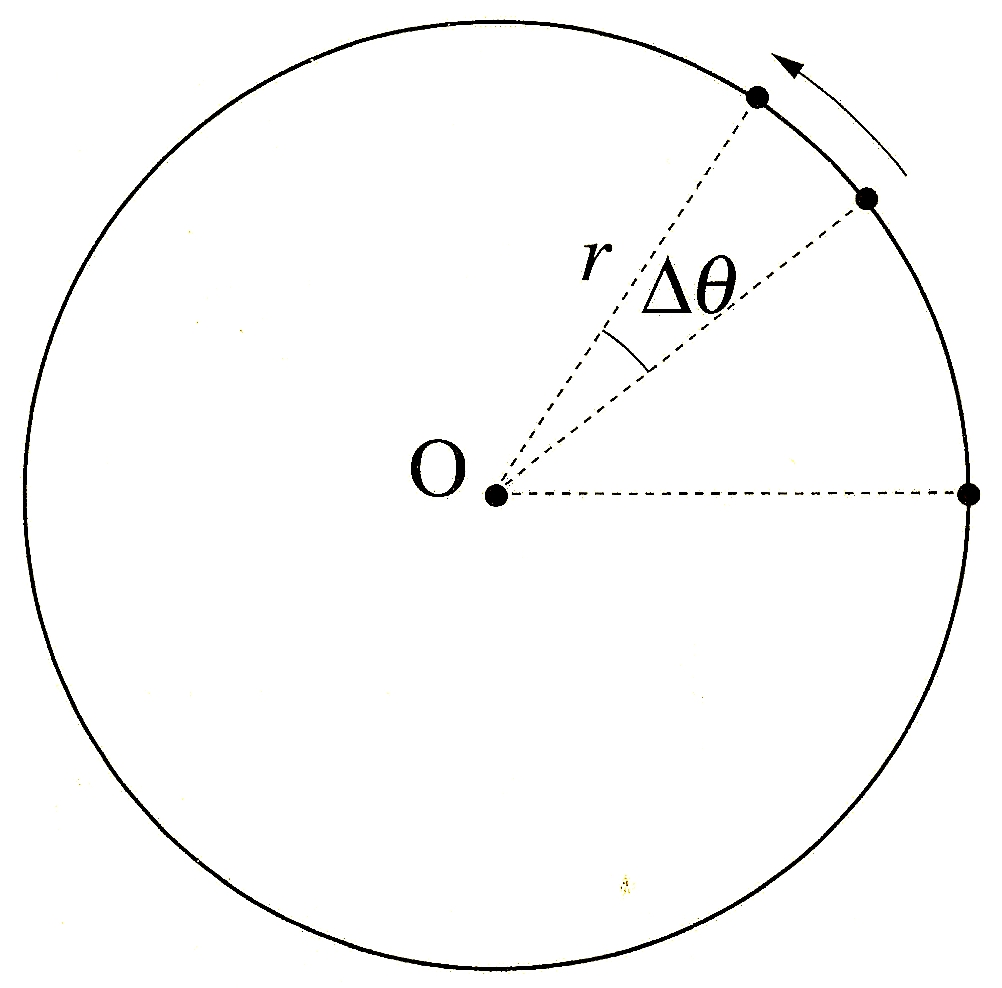
\includegraphics[width=0.35\textwidth]{ecb_hoeksnelheid}
\end{image}
Verschillende punten op je fietswiel hebben verschillende snelheden als hun afstand tot het centrum verschilt. 
Het ventieldopje moet immers in eenzelfde tijd meer afstand afleggen dan het sensortje van je snelheidsmeter. 
Toch bestaat het wiel uit één geheel. 
Als je naar de omwentelingshoek kijkt die een straal vanuit het centrum door een punt op het wiel maakt, dan is die voor alle punten gelijk. 
Hoe sneller het wiel draait, hoe groter ook de omwentelingshoek is die een straal gemaakt heeft. 
Daarom definiëren we de hoeksnelheid $\omega$ als de verandering van de omwentelingshoek tot de benodigde tijd.\footnote{De letter $\omega$ is de kleine letter van $\Omega$ en de laatste letter in het Griekse alfabet. Spreek $\omega$ uit als omega. Een $\omega$ is geen w, zoals ook een w geen $\omega$ is. O wee ($\omega$?) als je je op het examen in juni vergist \ldots}

\begin{equation*}
	\omega=\frac{\Delta\theta}{\Delta t}
\end{equation*}
De eenheid is radialen per seconde, $[\omega]=\rm rad/s$. Aangezien een volledige omwentelingshoek $2\pi$ bedraagt en de tijd nodig om rond te gaan de periode is, geldt
\begin{equation}
	\omega=\frac{2\pi}{T}=2\pi f\label{hoeksnelheid}
\end{equation}

\subsection{Kinematica van de cirkelbeweging}

We beschouwen een punt dat een cirkelbeweging maakt met straal $r$. We voeren een assenstelsel in met de oorsprong in het middelpunt van de cirkel.
\begin{image}
	\begin{tikzpicture}
		% Parameters
		\def\R{3}       % circle radius
		\def\ang{50}    % angle theta (degrees)
	  
		% Circle
		\draw (0,0) circle (\R);
	  
		% Axes
		\draw[->] (-\R-0.5,0) -- (\R+1,0) node[right] {$x$};
		\draw[->] (0,-\R-0.5) -- (0,\R+1) node[above] {$y$};

		\coordinate (O) at (0,0);
		\coordinate (A) at (\R,0);
	  
		\fill (0,0) circle (2pt) node[below left] {$O$};
	  
		% Point A on x-axis
		\fill (\R,0) circle (2pt) node[below right] {$A$};
	  
		% Point P on circle (polar coordinates)
		\coordinate (P) at (\ang:\R);
		\fill (P) circle (2pt) node[above right] {$(x,y)$};
	  
		% Radius vector r
		\draw[->] (0,0) -- (P) node[midway,above left] {$\vec{r}$};
	  
		% Dotted projections
		\draw[dashed] (P) -- (\ang:\R |- 0,0); % vertical projection
		\draw[dashed] (P) -- (\ang:\R -| 0,0); % horizontal projection
	  
		% Basis vectors e_x, e_y
		\draw[->] (0,0) -- (1.2,0) node[midway,below] {$\vec{e}_x$};
		\draw[->] (0,0) -- (0,1.2) node[midway,left] {$\vec{e}_y$};

		\pic [draw, pic text = $ \theta$, angle eccentricity=1.5] {angle = A--O--P};
	  
	  \end{tikzpicture}
	% 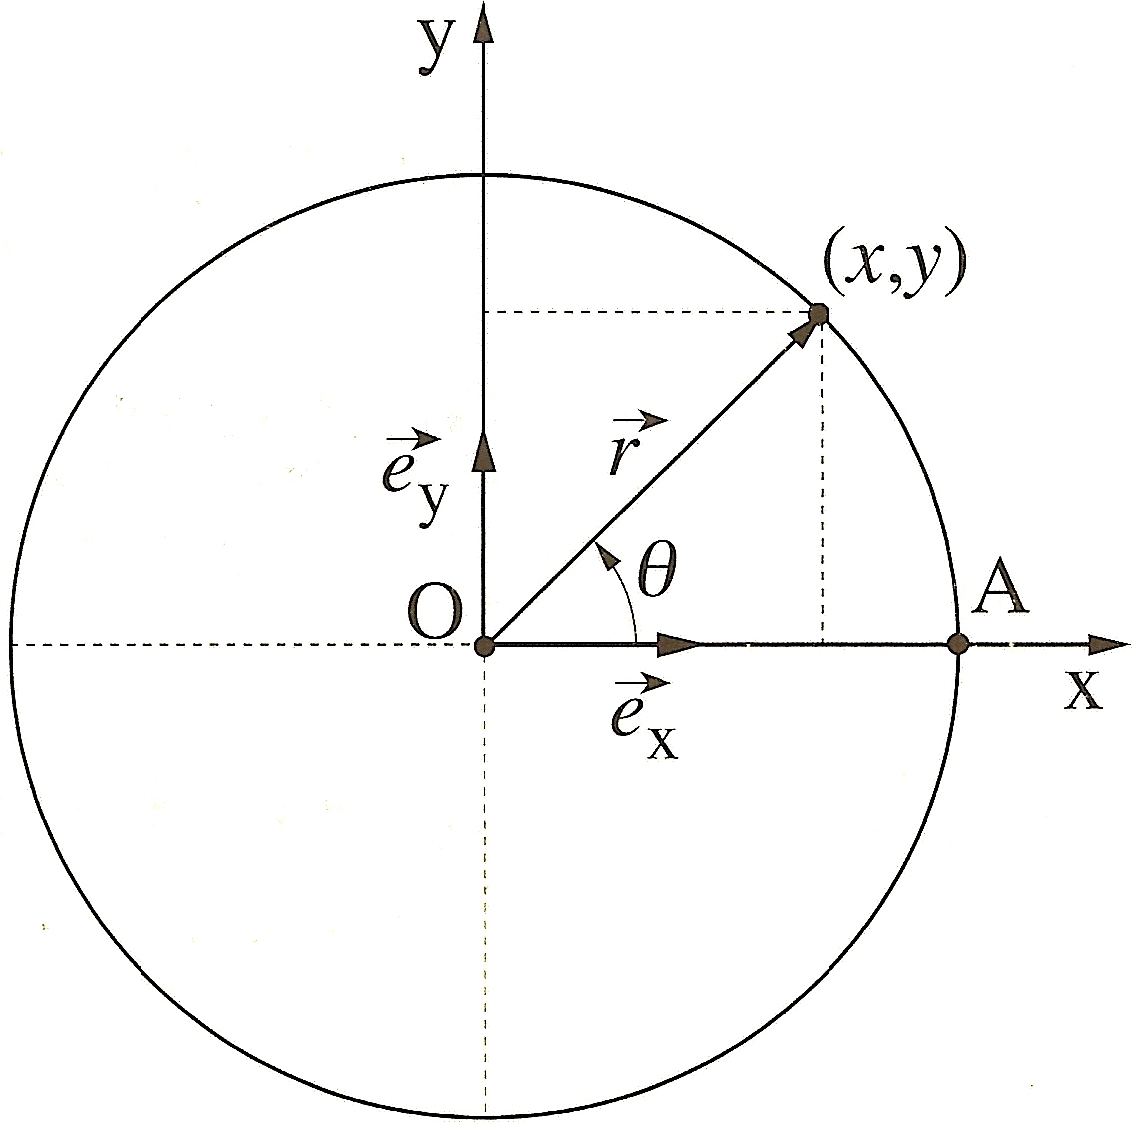
\includegraphics[width=0.4\textwidth]{ecb_positie}
\end{image}
Als we de omwentelingshoek $\theta$ meten vanaf de positieve $x$-as en en het tijdstip $t_0=0$ nemen, kunnen we de doorlopen omwentelingshoek als volgt in functie van de tijd schrijven.

\begin{equation*}
	\omega=\frac{\Delta\theta}{\Delta t}=\frac{\theta-\theta_0}{t-t_0} %=\frac{\theta}{t}\quad\Rightarrow\quad\theta=\omega t
\end{equation*}

Als we \(t_0 = 0\) nemen, komt \(\theta_0\) overeen met de starthoek. 
De formule herschrijven geeft dan voor de ECB een gelijkaardige formule als voor de eenparige rechtlijnige beweging (ERB).

\begin{equation*}
	\theta=\theta_0+\omega t
\end{equation*}
Voor de eenvoud nemen we meestal $\theta_0=0$ zodat $\theta=\omega t$. 



De coördinaatfuncties vinden we dan als projecties op de $x$- en $y$-as. \todo{klopt die term coördinaatfunctie wel?}
\begin{eqnarray*}
	x(t)&=&r\cos\omega t\\
	y(t)&=&r\sin\omega t
\end{eqnarray*}
We krijgen dan voor de plaatsvector, de snelheid en de versnelling:
\begin{eqnarray}
	\vec{r}&=&r\cos\omega t\cdot\vec{e}_x+r\sin\omega t\cdot\vec{e}_y\nonumber\\
	&\Downarrow&
	\left\{
		\begin{array}{l}
			v_x=\frac{dx}{dt}=-\omega r\sin\omega t\\
			v_y=\frac{dy}{dt}=\omega r\cos\omega t
		\end{array}
	\right.\nonumber\\
	\vec{v}&=&-\omega r\sin\omega t\cdot\vec{e}_x+\omega r\cos\omega t\cdot\vec{e}_y\nonumber\\
	&\Downarrow&
	\left\{
		\begin{array}{l}
			a_x=\frac{dv_x}{dt}=-\omega^2 r\cos\omega t\\
			a_y=\frac{dv_y}{dt}=-\omega^2 r\sin\omega t
		\end{array}
	\right.\nonumber\\
	\vec{a}&=&-\omega^2 r\cos\omega t\cdot\vec{e}_x-\omega^2 r\sin\omega t\cdot\vec{e}_y\nonumber\\
	&=&-\omega^2(r\cos\omega t\cdot\vec{e}_x+r\sin\omega t\cdot\vec{e}_y)\nonumber\\
	&\Updownarrow&\nonumber\\
	\vec{a}&=&-\omega^2\vec{r}\label{versnelling}
\end{eqnarray}

Deze laatste gelijkheid is zeer belangrijk. We vinden dat de versnelling steeds naar het middelpunt van de cirkel is ge\"ori\"enteerd \ldots! We noemen het bijgevolg een centripetale\footnote{Dit is niet hetzelfde als centrifugaal.} of middelpuntzoekende versnelling.

\begin{image}
	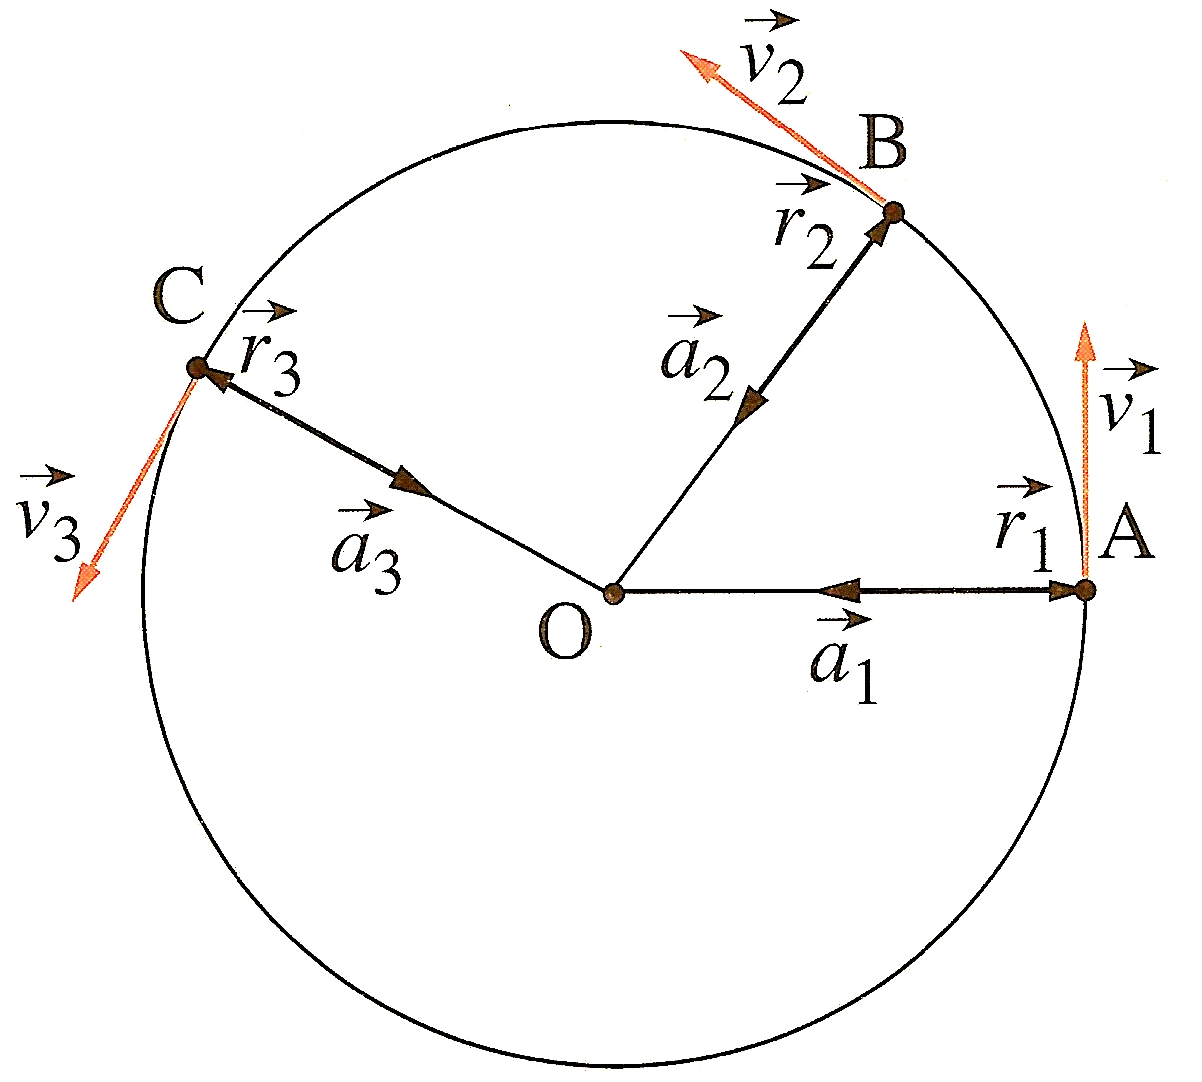
\includegraphics[width=0.4\textwidth]{ecb_versnelling}
\end{image}

Je zou dit resultaat opmerkelijk kunnen noemen aangezien de snelheid een constante grootte heeft.
Maar tegelijk ook niet omdat we hier te maken hebben met een richtingsveranderende versnelling, de normale versnelling uit het hoofdstuk basisbegrippen.

\begin{eqnarray}
	v=\parallel\vec{v}\parallel&=&\sqrt{v_x^2+v_y^2}\nonumber\\
	&=&\sqrt{(-\omega r\sin\omega t)^2+(\omega r\cos\omega t)^2}\nonumber\\
	&=&\sqrt{r^2\omega^2(\sin^2\omega t+\cos^2\omega t)}\nonumber\\
	&\Updownarrow&\nonumber\\
	v&=&r\omega\label{snelheid}
\end{eqnarray}

 Verandert de richting van de snelheid en aangezien versnelling de verandering van de snelheid is, moet er een versnelling zijn. 
 Deze is naar het centrum ge\"ori\"enteerd omdat een fractie van een seconde later het object -- in vergelijking met de rechte baan die het zou afleggen moest het volgens de snelheid die het op een bepaald moment heeft, voortbewegen -- iets dichter naar het centrum moet zijn gekomen. 
 De snelheidsvector is in grootte niet veranderd maar wel gedraaid, in de richting van het centrum. 
 Moest bovendien de versnelling niet loodrecht op de snelheid staan, dan zou de versnelling een component volgens de snelheid hebben wat zou betekenen dat de snelheid in die richting zou moeten veranderen van grootte.

\begin{image}
	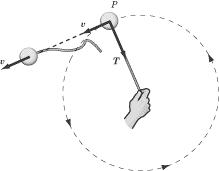
\includegraphics[width=0.4\textwidth]{ballnostring}
\end{image}
Toelichting figuur: Moest er geen versnelling naar het centrum zijn -- bv. in het geval dat een touwtje met een ronddraaiend object aan, knapt -- dan zou de snelheid niet veranderen en het object op een rechte baan in het verlengde van de snelheid met een constante snelheid voortbewegen.

Uit (\ref{hoeksnelheid}), (\ref{versnelling}) en (\ref{snelheid}) vinden we nog:
\begin{equation}
	a=r\omega^2=v\omega=\frac{v^2}{r}
\end{equation}
Merk op dat de snelheid een kwadratische invloed op de grootte van de versnelling heeft.

\end{document}
